\documentclass[tikz, border={0pt 0pt 0pt 6pt}]{standalone}
\usetikzlibrary{arrows,decorations.markings}
\usetikzlibrary{arrows.meta}% CVS
\begin{document}
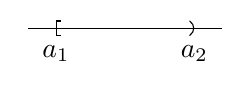
\begin{tikzpicture}[inner sep=+0pt]
  \draw (+0pt,+0pt) -- ++(right:+10pt) coordinate (@);
  \draw[[-)] (@) node[below=+6pt] {$a_1$} -- ++ (right:+50pt) node[below=+6pt] {$a_2$} coordinate (@);
  \draw (@) -- ++ (right:+10pt);
\end{tikzpicture}

\tikz[inner sep=+0pt, outer sep=+0pt, nodes={below=+6pt}]
  \draw[decoration={
    markings, mark=at position .2 with {\arrow[line width=.7\pgflinewidth,scale=2]{[}},
              mark=at position .8 with {\arrow[line width=.7\pgflinewidth,scale=2]{)}}},
        postaction=decorate]
    (+0pt,+0pt) -- node[pos=.2, below=+3pt] {$a_1$} node[pos=.8, below=+3pt] {$a_2$} ++(right:+70pt);


\tikz[label position=below, inner sep=+0pt, outer sep=+0pt, every label/.style={font=},
  label distance=+3pt, nodes={font=\bfseries}]
  \draw (+0pt,+0pt) -- node[pos=.2,label=$a_1$] {[} node[pos=.8,label=$a_2$] {)} ++(right:+70pt);

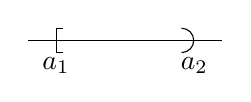
\begin{tikzpicture}[inner sep=+0pt, arrows={[scale=2]}]% CVS
  \draw (+0pt,+0pt) -- ++(right:+10pt) coordinate (@);
  \draw[Bracket-Arc Barb] (@) node[below=+6pt] {$a_1$} -- ++ (right:+50pt) node[below=+6pt] {$a_2$} coordinate (@);
  \draw (@) -- ++ (right:+10pt);
\end{tikzpicture}
\end{document}